The models were evaluated on two standard datasets, videos of bouncing balls and motion capture data, and compared to the RNN-RBM and RTRBM models discussed in Chapter 2 (Related Work) as well as an LSTM.

\section{Samples from RNN-RBM on sequenced MNIST}

Compared to the samples generated by the RNN-RBM, it is clear that the GSN framework has an easier time mixing between modes of the input data. It also appears to form better reconstructions of the input data. This improvement can be attributed to a deeper representation of the input space, since the RNN-RBM only had two layers - one for the RBM and one for the RNN.

\begin{figure}[h!]
  \centering
    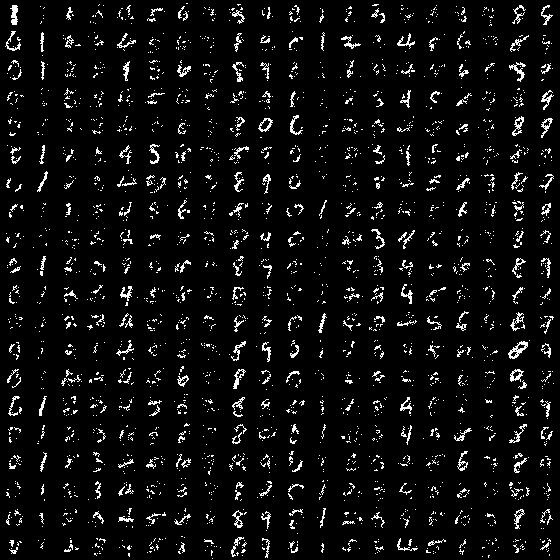
\includegraphics[width=0.8\textwidth]{rnnrbm_samples}
\caption{RNN-RBM sampling after 300 iterations.}
\end{figure}

\section{Bouncing balls videos dataset}

This dataset generates videos of 3 balls bouncing and colliding in a box as described in \cite{lewandowski12}\footnote{http://www.cs.utoronto.ca/~ilya/code/2008/RTRBM.tar}. The videos have length of 128 frames with 15x15 resolution of pixels in the range of [0, 1]. Training examples are generated artificially at runtime so each sequence seen is unique, which helps reduce overfitting.

The LSTM and Untied GSN models were trained with two layers of 500 hidden units. The Temporal GSN used two layers of 500 units with tied weights, input salt-and-pepper noise of 0.2, hidden Gaussian noise of 0 mean and 1 standard deviation, 4 walkback steps, and a history context window of 4 timesteps. The RNN-GSN had two GSN layers of 500 units with tied weights and 4 walkbacks, and a single layer LSTM with 500 hidden units. The SEN had two GSN layers and two LSTM layers, where the GSN had 2 layers of 500 hidden units with tied weights and 4 walkback steps, and the LSTM had 500 hidden units.

All models were trained on subsequences with length 100 using the Adam optimizer with a learning rate of 0.001, beta1 of 0.9, and beta2 of 0.999. Gradients were scaled to clip the batchwise L2 norm at a maximum of 0.25.


\section{CMU motion capture dataset}

This dataset is a series of captured human joint angles, translations and rotations around the base of a spine as in \cite{sutskever08}\footnote{https://github.com/sidsig/NIPS-2014}. There are 3826 samples of 49 real-valued inputs, so input sampling was not used for the GSN and the visible layer had a linear activation.

The train set was split as the first 80\% of each sequence, with the last 20\% forming the test set.

The LSTM and Untied GSN models were trained with two layers of 128 hidden units. The Temporal GSN used two layers of 128 units with tied weights, input salt-and-pepper noise of 0.1, hidden Gaussian noise of 0 mean and .5 standard deviation, 4 walkback steps, and a history context window of 3 timesteps. The RNN-GSN had two GSN layers of 128 units with tied weights and 4 walkbacks, and a single layer LSTM with 256 hidden units. The SEN had two GSN layers and two LSTM layers, where the GSN had 2 layers of 128 hidden units with tied weights and 4 walkback steps, and the LSTM had 128 hidden units.

All models were trained on subsequences with length 100 using the Adam optimizer with a learning rate of 0.001, beta1 of 0.9, and beta2 of 0.999. Gradients were scaled to clip the batchwise L2 norm at a maximum of 0.25.

\begin{table}[h!]
\begin{tabular*}{\textwidth}{p{4cm} r r r r}
\hlinewd{1.5pt}
  & Bouncing Balls & CMU Motion Capture \\
\hline
LSTM & \bfseries0.11 & 9.24\\
RTRBM & 2.11 & 20.1\\
RNN-RBM & 0.96 & 16.2\\
Untied GSN & 0.94 & \bfseries6.90\\
TGSN & 5.57 & 9.27\\
RNN-GSN & 5.28 & 11.49\\
SEN & 19.0 & 50.8\\
\hlinewd{1.5pt}
\end{tabular*}
\caption{Mean squared prediction error on bouncing balls videos and motion capture data. RTRBM and RNN-RBM numbers from [10]}
\end{table}

\section{Results}
Notably, the baseline LSTM outperformed all other models on the videos of bouncing balls dataset, achieving a mean frame-level square prediction error of 0.11. The Untied GSN had lower error than the RNN-RBM, but the TGSN and RNN-GSN both did much worse. One possible explanation is the EM algorithm entered bad RNN state transitions as discussed in Chapter 5.3. This can be seen in the RNN-GSN frame outputs, which diverged from a good state into a bad representation. Another reason the GSN-based models (except the Untied GSN) performed poorly is the injected salt-and-pepper and gaussian noise remaining relatively high throughout the process. We would like to explore noise scheduling in the future to help training convergence.

\begin{figure}[h!]
  \centering
    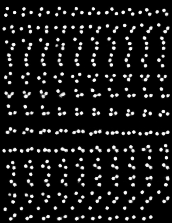
\includegraphics[width=0.3\textwidth]{bouncing_rnngsn_12}
\caption{RNN-GSN good state.}
\end{figure}

\begin{figure}[h!]
  \centering
    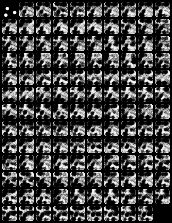
\includegraphics[width=0.3\textwidth]{bouncing_rnngsn_32}
\caption{RNN-GSN diverged bad state.}
\end{figure}

For the CMU motion capture dataset, the Untied GSN model had the lowest mean frame-level square prediction error at 6.90. The LSTM and TGSN were similar in error and all other models except the SEN outperformed the RTRBM and RNN-RBM baselines. This dataset has a much lower input dimensionality, so we are less likely for the optimization to diverge using the GSN-based models. Further, the added noise for GSNs were lower in this experiment than in the bouncing balls video dataset.

Ultimately the SEN in both experiments was not able to converge. We believe learning reconstructions of higher-level sequence representations without those representations being in a relatively stable starting point leads to high training instability. Future work will explore layer-wise pretraining, or dynamically growing the number of layers to encourage representation stability and training convergence. Further hyperparameter search for learning rate and gradient clipping should also be performed to help stability.

\begin{figure}[h!]
  \centering
    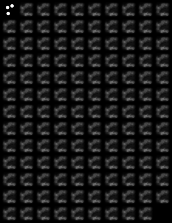
\includegraphics[width=0.3\textwidth]{bouncing_sen_140}
\caption{SEN frame predictions after 140 epochs.}
\end{figure}

\section{Future Work}
Future work will focus on studying the Sequence Encoder Network class of architectures and their training stability. We would like to explore convolutional autoencoders for image-based prediction tasks, and sequence-to-sequence models for language tasks, with GRU's as recurrent layers. Future work should also explore using adversarial loss during reconstruction to help stability and avoid mode collapse over sequences.

